\section{Performance Evaluation}
\label{sec:experiments}
\subsection{Implementation}

% Object models, constructed using the kinect fusion algorithm from PCL, were used to construct $B_0$. The performance of the static and the active detectors were compared on synthetic scenes obtained from $B_0$. The results are summarized in Subsection \ref{subsec:static_v_active}. In Subsection \ref{subsec:real_scene}, the active framework was evaluated on several real scenes from a lab environment captured with a kinect sensor.
% 
% We used a subset of $10$ models from $B_0$ and $2$ clutter models to define $B_1$. Templates were extracted from them and were used to train the vocabulary tree. A single object of interest was used: $B_2 = \{\text{Handlebottle}\}$. The space of object yaws was discretized into $6$ bins to formulate hypotheses about the detections:
% \begin{align*}
% H_0 =& \text{ The object is \textit{not} a Handlebottle}\\
% H_i =& \text{ The object is a Handlebottle with yaw $(i-1)60$ deg}\\
% 	 &\quad\text{for } i=1,\ldots,6 
% \end{align*}
% 
% 
% \subsection{Static versus active object detection}
% \label{subsec:static_v_active}
% Fourteen synthetic scenes with $5$ objects each were constructed from the models in $B_0$. The objects were chosen so that there were $10$ instances of each hypothesis. The active detection algorithm was used with a simulated depth sensor to make decisions. Twenty five repetitions with different starting sensor poses were carried out for very object. The score from the vocabulary tree after the first observation was recorded as the decision of the static detector. The results are summarized in Fig. \ref{fig:confusion_matrix}.
% \begin{figure}[ht!]
% 	\centering
% 	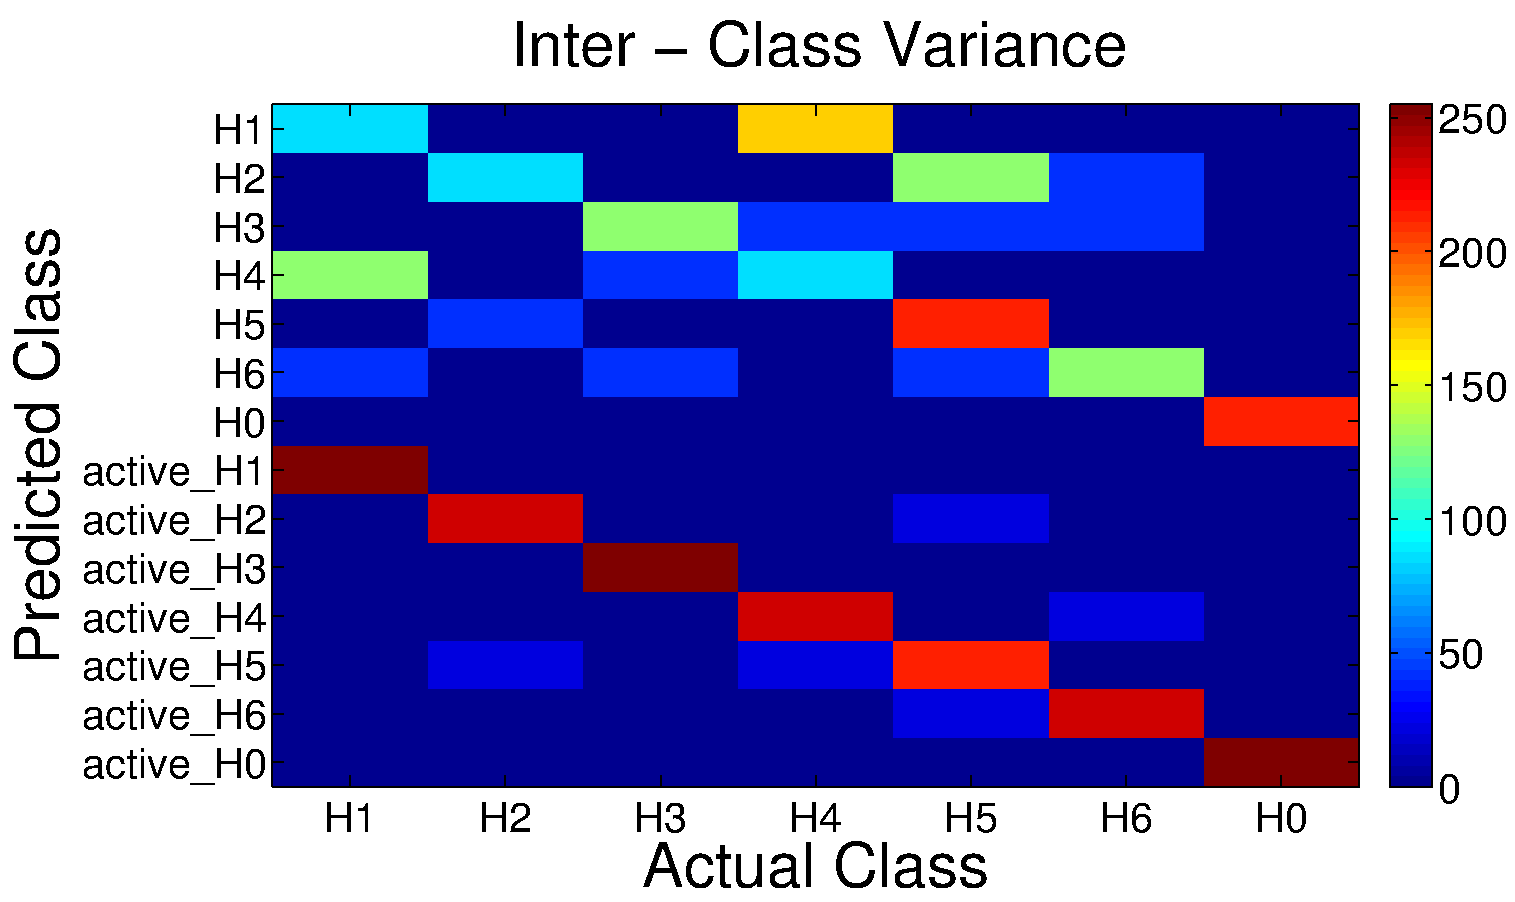
\includegraphics[width=\linewidth]{figs/active.pdf}
% 	\caption{Confusion matrix comparing the performance of the static and the active object detectors. The columns show the true hypotheses associated with each detection. The first $7$ rows present the decisions made by the static detector. The last $7$ rows show the decisions made by the active detector}
% 	\label{fig:confusion_matrix}
% \end{figure}
% The first seven rows of the confusion matrix show the decisions of the static object detector, while the results from the active framework are shown in the last seven rows. There is a marked improvement in the results when the active detection module is used.
% 
% \subsection{Experiments with real scenes}
% \label{subsec:real_scene}
% Several real scenes were captured from our lab using a kinect sensor and the fusion algorithm from PCL (See Fig. \ref{real_scene:color}). With $B_2$ and $B_1$ the same as before, the sensor's task was to detect any Handlebottles on the table and estimate their orientation. The opreration of the active detection algorithm is exemplified in Fig. \ref{real_scene:active_framework}. Since the object orientations in a real scene are not discretized a refinement step is needed if the algorithm detects an object of interest, i.e. decides on $H_i, i>0$. Then, the last observed pointcloud is aligned with the database template, which corresponds to $H_i$ using an iterative closest point algorithm. Thus, the final decision includes both a class and a continuous pose estimate.
% 
% The algorithm colors the pointcloud clusters based on its current understanding of them. Objects, which have been seen but not processed yet are colored red. The object, which is currently under evaluation is colored yellow. Once the system makes a decision about an object, it is colored green if it is of interest, i.e. in $B_2$, and blue otherwise. Fig. \ref{real_scene:result} shows a detected Handlebottle in the scene. The active framework chose hypothesis $H_3$, which corresponds to a yaw of $120\degree$. The model associated with $H_3$ is overlaid on the scene \textit{before} the orientation refinement. As you can see the two objects are already very close and the alignment procedure will produce a good \textit{continuous} orientation estimate.
% \begin{figure*}[ht!]
%   \begin{center}
%     \subfigure[Real scene captured using kinect fusion]{\label{real_scene:color}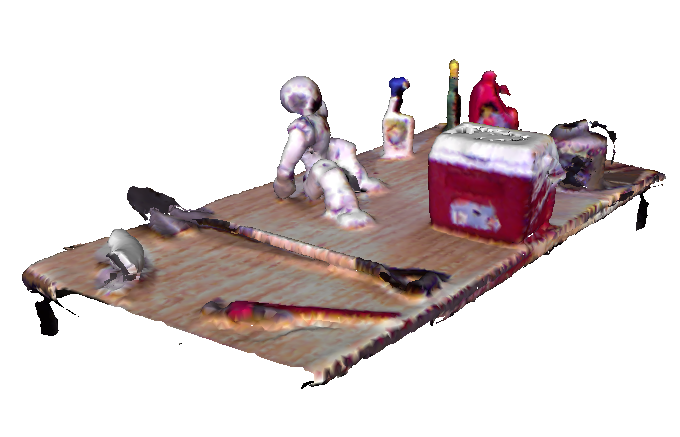
\includegraphics[width=57mm]{figs/1_real_scene.png}} 
%     \subfigure[Our algorithm's interpretation of the scene]{\label{real_scene:active_framework}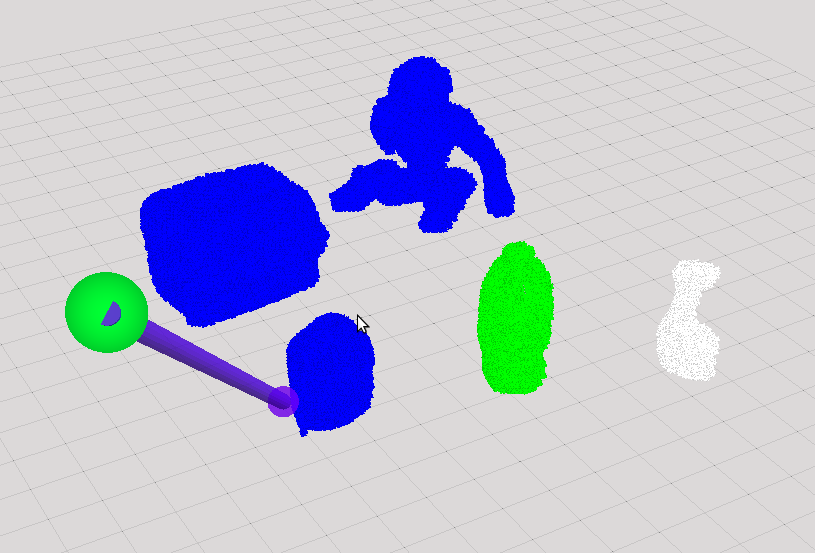
\includegraphics[width=57mm]{figs/2_decision_profile.png}}
%     \subfigure[The object of interest is detected]{\label{real_scene:result}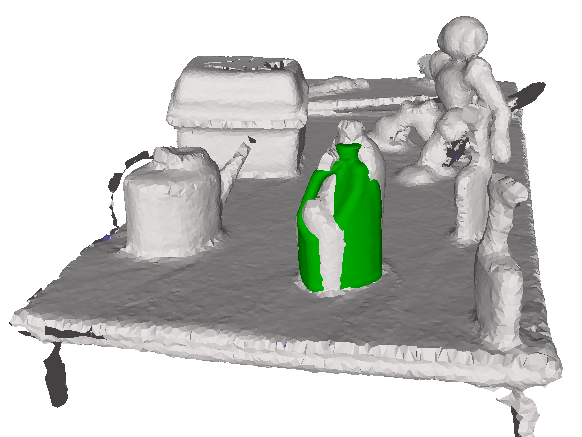
\includegraphics[width=57mm]{figs/3_final_detection.png}}
%   \end{center}
%   \caption{The active detection framework is applied to a real scene. An object is colored green if the algorithm decides it is of interest (in $B_2$) and blue otherwise. Hypothesis 3 (Handlebottle with yaw $120\degree$) was chosen for the green object in Fig. \ref{real_scene:active_framework}. The model associated with $H_3$ is overlaid on the scene in Fig. \ref{real_scene:result}  \textit{before} the final orientation refinement. See the attached video or \protect\url{http://www.seas.upenn.edu/~atanasov/ICRA2013_ActivePerception.mp4} for more details.}
%   \label{fig:real_scene}
% \end{figure*}
% 
% 
% 


%Three sets of experiments were carried out in order to evaluate the performance of our framework. Object models were constructed using a kinect sensor and were divided in testing and training classes as follows:
%\begin{align*}
%B_0 =& \{\text{Axe, Bigbox, Broom, Brush, Flowerspray, Gastank,}\\
%&\quad\text{Handlebottle, Heavyranch, Pan, Pipe, Shovel,}\\
%&\quad\text{Spadefork, Spraybottle, Watercan, Wreckbar, Robot}\}\\
%B_1 =& \{\text{Bigbox, Brush, Flowerspray, Handlebottle, Pan,}\\
%&\quad\text{Heavyranch, Pipe, Shovel, Spraybottle, Watercan}\}\\
%B_2 =& \{\text{Handlebottle}\}\\
%\end{align*}

%The object classes from $B_0$ were used to construct $14$ synthetic test scenes as described in Section \ref{sec:problem}. The performances of the static and the active object detectors were compared on all test scenes. Finally, we performed experiments using real scenes captured with the kinect sensor.















%\subsection{Evaluation of the static detector}
%\subsection{Evaluation of the active detector ion framework}
%active detection: For 14 testing scenes, run the detection thing and see the final hypotheses. Check if yaw is correct


%Our vocabulary tree is trained on templates extracted from each of these possible pose hypotheses for our object of interest. It also consists various pose templates that correspond to other objects from a limited database of objects. The tree we train has more than 1 million nodes corresponding to 11 object classes and six possible pose
%hypotheses for each class, namely from zero to 300 degrees yaw discretized at intervals of 60 degrees. In our experiements we specifically try to detect an object of class ``handlebottle'' with randomn yaw. When the vocabulary tree is queried by the active detection module, it returns a seven bit indicator
%vector corresponding to the best retreival from the vocabulary tree. For instance if the best retreival is of the ``handlebottle'' class of yaw 120 degrees then the bit corresponding to hypothesis H3 is turned on and the rest are set to zero. If the best retreival does not belong to the ``handlebottle'' class we
%set the first bit in the hypothesis indicator vector to on, i.e the bit corresponding to the zero hypothesis.
%We then use the observation model to update our posterior of the current cluster with the likelihood of this observation from the current viewpoint. In the strictly active detection case, if the final hypothesis corresponds to one of the pose hypotheses of the "handlebottle" class we use that pose hypothesis to perform a coarse to fine refinement for our final pose estimate.  

%In scenarios where the task completion hinges on the robot's ability to classify it's environment accurately based on its perceptual sensor modalities, an incorrect classification by a static object detector can adversely affect the outcome of the task. Instead in the active object
%detection scenario we let the robot move in its environment to verify its current hypothesis before performing the next task. To evaluate the comparative performance of these approaches we evaluated the output of our static object detector against the output produced by our
%active detection strategy.
%In a use case experiment we take a test scene where we are looking for a object of a specific class amongst a set of randomnly placed objects on a table. We take a scene consisting of randomly distributed objects. With our static detection pipeline we can query the vocabulary tree to get the closest template to the current surface being viewed by 
%the sensor.  These objects can consist of object classes that our vocabulary tree has been trained on and those that have never been seen before by the classifier. The pipeline is setup such that given an input scene the algorithm first extracts
%clusters above a planar surface, followed by which we update our posterior for each cluster given the data likelihood generated by the observation model. Using these posteriors we order the clusters in a priority queue and classify each cluser starting from the most likely cluster, all the way to the 
%cluster that is least likely of being the object of interest.
%We have a set of seven hypothesis of each cluster, one hypothesis corresponding to the cluster not belonging to the object class that we are trying to detect. The rest of the hypotheses correspond to the various possible coarse pose estimates of the object.






%%\begin{figure}
%%\centering
%%\subfigure{
%%	\label{sub:real_scene}
%%	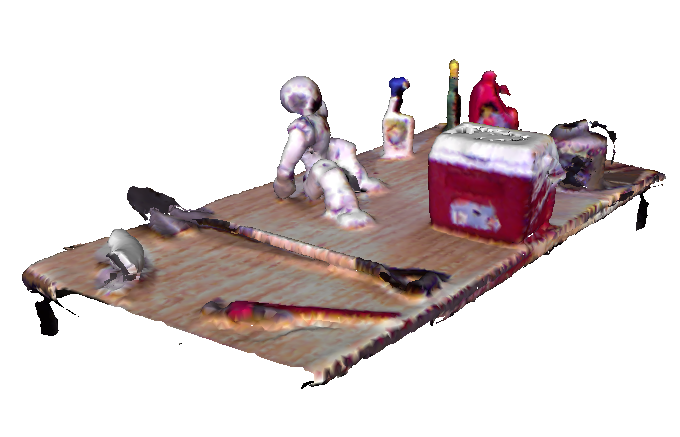
\includegraphics[width=\linewidth]{figs/real_scene_crop.png}
%%	\caption{Real scene obtained from a kinect sensor}
%%}
%%\subfigure{
%%	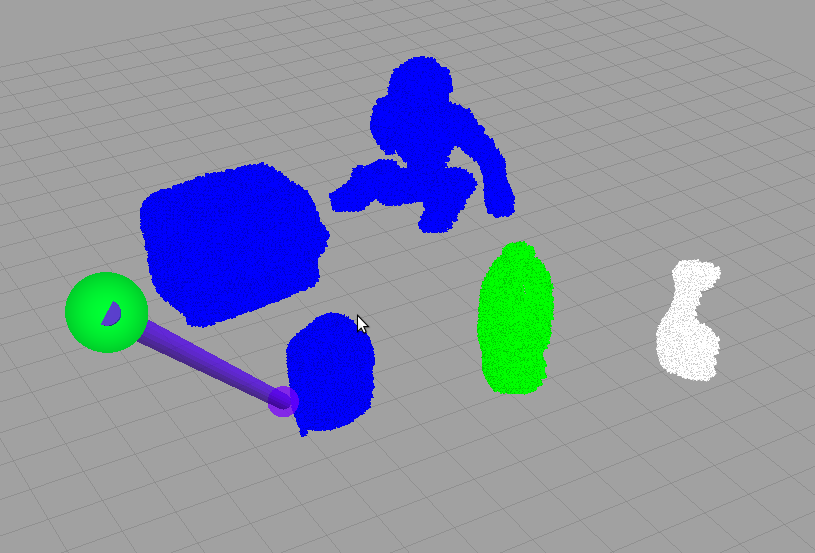
\includegraphics[width=\linewidth]{figs/decision_profile2.png}
%%	\caption{Final detections for the objects in \ref{sub:real_scene}. Blue represents non-bottle objects; green represents detected bottles. }
%%}
%%\caption{An experiment peformed using a scene captured by a kinect sensor, The top scene is the output using the kinect and the bottom images is the classification using the active detection pipeline}
%%\label{fig: scarab}
%%\end{figure}


%\subsection{Static Object Detection}
%%efficiency of our vocabulary tree by analyzing the inter-intra class variance.
%%Fig \ref{fig:templates_intra} below shows the performance of the object detection algorithm when we test for performance accuracy with respect to every template encoded.
%Our vocabulary tree is trained on templates extracted from each of these possible pose hypotheses for our object of interest. It also consists various pose templates that correspond to other objects from a limited database of objects. The tree we train has more than 1 million nodes corresponding to 11 object classes and six possible pose
%hypotheses for each class, namely from zero to 300 degrees yaw discretized at intervals of 60 degrees. In our experiements we specifically try to detect an object of class ``handlebottle'' with randomn yaw. When the vocabulary tree is queried by the active detection module, it returns a seven bit indicator
%vector corresponding to the best retreival from the vocabulary tree. For instance if the best retreival is of the ``handlebottle'' class of yaw 120 degrees then the bit corresponding to hypothesis H3 is turned on and the rest are set to zero. If the best retreival does not belong to the ``handlebottle'' class we
%set the first bit in the hypothesis indicator vector to on, i.e the bit corresponding to the zero hypothesis.
%We then use the observation model to update our posterior of the current cluster with the likelihood of this observation from the current viewpoint. In the strictly active detection case, if the final hypothesis corresponds to one of the pose hypotheses of the "handlebottle" class we use that pose hypothesis to perform a coarse to fine refinement for our final pose estimate.  

%\subsection{Hypothesis Testing for Active Object Detection}
%\label{sec:experiments}
%In our active detection strategy, as we update our posterior based on the likelihood of the observation given by the model, our active detection module either tries to take a new observation or decide on the best hypothesis. We make a decision for a cluster based on the balance betweem the cost for making a mistake and the cost of moving to an other viewpoint to get a new observation.
%In the attached video \url{:http://www.seas.upenn.edu/~atanasov/ICRA2013_ActivePerception}, if a cluster has no decision associated with it, it is colored red. When the algorithm is deciding on a cluster it is colored yellow. If it is determined to be a handlebottle the cluster color is updated
%to green if the algorithm decides on the zero hypothesis, the culster color changes to blue.

%In the figure below Fig ~\ref{fig:templates_intra}, you can see that our active detection module outperforms a static detection setup we. Tested our approach on 20 test scenes generated using a kinect and a set of random objects placed on a table.


%To study interclass variance we compare the document retreival efficiency with the best template of each class of objects and not just the best overall template as we saw in the previous experiment.
%\begin{figure}[ht!]
%	\centering
%	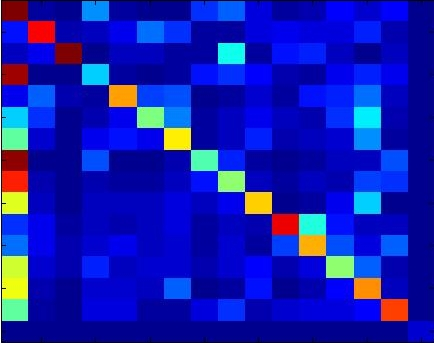
\includegraphics[height=5cm]{figs/interclass_variance.jpg}
%	\caption{Confusion Matrix for all classes in the Tree, Rows are the active and static detection outputs, Columns are the actual classes}
%	\label{fig:templates_inter}
%\end{figure} 
%As it can be noted the interclass variance is more distinct albeit there are some classes that are not accurately classified and yield false positive.




%\begin{figure}[h]
%\begin{center}$
%\begin{array}{ccc}
%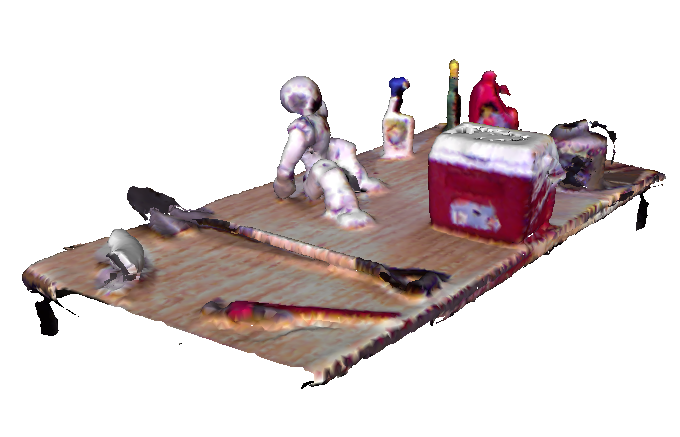
\includegraphics[width=0.3\linewidth]{figs/real_scene_crop.png} &
%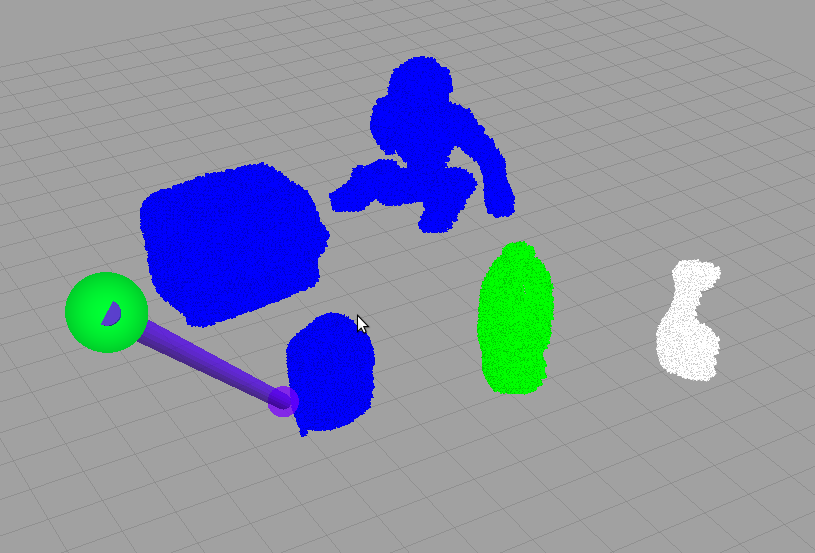
\includegraphics[width=0.3\linewidth]{figs/decision_profile2.png} &
%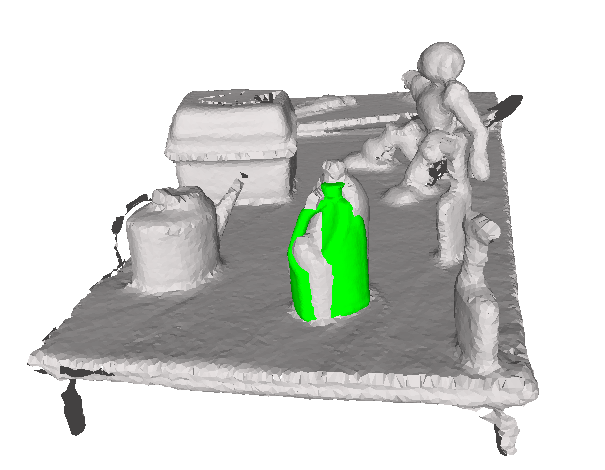
\includegraphics[width=0.3\linewidth]{figs/final_transformation.png}
%\end{array}$
%\end{center}
%\caption{my caption}
%\end{figure}






%Once a decision is made for the current cluster, the sensor moves to the next cluster in the priority queue. During the detection phase we keep a history of the estimated pose of the object returned by the coarse to fine pose refinement algorithm. We also retain a history of the visited positions in the scene to ensure that the algorithm does not oscillate between local optima.



%\begin{algorithm}[H]
%\caption{Active object detection pipeine}
%\label{pscode:pipeline}
%\begin{algorithmic}[1]
%\footnotesize
%\State \textbf{Input}: Point cloud $\mathbb{Q}$
%\State \textbf{Output}: Decision Profile $\mathbb{D}$
%\State get pointlcoud $\mathbb{Q}$ for the scene
%\State cluster $\mathbb{Q}$ into {\it k} clusters
%\State $\forall \mathbb{Q}_k \in \mathbb{Q}$ get a new sensor reading with the sensor pointed towards its centroid
%\State score the new surface $\mathbb{Q}_k$ using vocabulary tree to get $H_{0_k}$
%\State sort all $H_{0_k} \in \mathbb{Q}$ into a priority queue $\mathbb{P}$
%\State \textbf{For}: $\forall \mathbb{Q}_k \in \mathbb{P}$
%\State   Compute policy
%\State    \textbf{While}:{ best action $!=$ DECIDED}
%\State       Execute best action
%\State       Get new sensor measurement $\mathbb{Q}_k$
%\State       Update belief $H_{0_k}$
%\State   \textbf{End While}
%\State \textbf{End For}
%\end{algorithmic}
%\end{algorithm}


% \begin{algorithm}[ht]
% \caption{Active object detection pipeine}
% \label{pscode:pipeline}
% \begin{algorithmic}[1]

% \STATE {\bf Input:} Viewed Surface $s$, Object Models $\mathscr{M}_0$ and $\mathscr{M}_1$
% \STATE {\bf Output: Optimal Action: $\mathbb{A}$}
% \STATE
% \STATE $\text{Compute Model Hypothesis from Template Alignment scores for } \{s,\mathscr{M}_i\}$
% \STATE $\text{Construct octree } \mathscr{O}_i \text{ and label for each model } \mathscr{M}_i$
% \STATE Discretize viewsphere and compute set of viewpoints $\mathscr{V}$
% \FOR {$\forall v_i \in \mathscr{V}$}
% \STATE {Compute information gain $I.G(v_i)$}
% \ENDFOR 
% \STATE{\bf end for} 
% \STATE
% \STATE Compute Optimal Action $\mathbb{A}$ by solving F-HASHT
% \STATE
% \STATE{{\bf return} $\mathbb{A}$}
% \end{algorithmic}
% \end{algorithm}
